\newcommand{\flooderTagResultsAucTable}{
    \begin{table}[H]
        \centering
        \begin{tabular}{|p{2,8cm}||P{2,4cm} P{2,4cm} P{2,4cm}|}
            \hline
            Flooder Tag & ALOHA\newline (M/B only) & ALOHA & Proposed\newline Model \\
            \hline
            AUC-ROC & - & 0.985$\pm$0.001 & \textBF{0.985$\pm$0.000} \\
            \hline
        \end{tabular}
        \caption[Flooder Tag prediction task AUC-ROC results]{AUC-ROC (Area Under Curve) of the different models for the \textbf{Flooder Tag} prediction task. Results were aggregated over \textBF{2} training runs with different weight initializations and minibatch orderings. Best results are shown in \textbf{bold}.} \label{tab:flooderTag_auc}
    \end{table}
}

\newcommand{\flooderTagResultsAtFprTable}{
    \begin{center}
        \begin{longtable}[c]{|P{3,2cm}||P{1,8cm} P{1,8cm} P{1,8cm} P{1,8cm} P{1,8cm}|}
            \hline
            Flooder Tag & \multicolumn{5}{c|}{{FPR}} \\
            & $10^{-5}$ & $10^{-4}$ & $10^{-3}$ & $10^{-2}$ & $10^{-1}$ \\
            \hline
            \endfirsthead

            \caption*{\raggedright ...continued from previous page} \\
            \hline
            Flooder Tag & \multicolumn{5}{c|}{\textbf{FPR}} \\
            & $10^{-5}$ & $10^{-4}$ & $10^{-3}$ & $10^{-2}$ & $10^{-1}$ \\
            \hline
            \endhead

            \caption*{\raggedleft ...continued on next page} \\
            \endfoot

            \caption[Flooder Tag prediction task results]{Mean and standard deviation results (TPR, Accuracy, Recall, Precision and F1-Score) of the different models for the \textbf{Flooder Tag} prediction task at different \textbf{FPR}s (\textit{False Positive Rates}). Results were aggregated over \textBF{2} training runs with different weight initializations and minibatch orderings. Best results are shown in \textbf{bold}. Under \textbf{TPR} results are also presented the percentage reduction in mean detection error and in ROC curve standard deviation introduced by the \textit{Proposed Model} with respect to both \textit{ALOHA} model and \textit{Joint Embedding}.} \label{tab:flooderTag_results_at_fpr} \\
            \endlastfoot

            \multicolumn{6}{|c|}{\textbf{TPR}} \\
            \hline
            ALOHA (M/B only) & - & - & - & - & - \\
            ALOHA & 0.821$\pm$0.004 & \textBF{0.846$\pm$0.002} & \textBF{0.865$\pm$0.007} & 0.904$\pm$0.002 & 0.953$\pm$0.005 \\
            Proposed Model & 0.817$\pm$0.005 & 0.818$\pm$0.006 & 0.818$\pm$0.006 & \textBF{0.905$\pm$0.002} & \textBF{0.965$\pm$0.001} \\
            \hline
            Error Reduction wrt\newline ALOHA (M/B only) & - & - & - & - & - \\
            Error Reduction wrt\newline ALOHA & -2.2\% & -18.2\% & -34.8\% & 1.0\% & 25.5\% \\
            \hline
            Std Reduction wrt\newline ALOHA (M/B only) & - & - & - & - & - \\
            Std Reduction wrt\newline ALOHA & -25.0\% & -200.0\% & 14.3\% & 0.0\% & 80.0\% \\
            \hline
            \multicolumn{6}{|c|}{\textbf{Accuracy}} \\
            \hline
            ALOHA (M/B only) & - & - & - & - & - \\
            ALOHA & \textBF{1.000$\pm$0.000} & \textBF{1.000$\pm$0.000} & \textBF{0.999$\pm$0.000} & \textBF{0.990$\pm$0.000} & \textBF{0.900$\pm$0.000} \\
            Proposed Model & \textBF{1.000$\pm$0.000} & \textBF{1.000$\pm$0.000} & \textBF{0.999$\pm$0.000} & \textBF{0.990$\pm$0.000} & \textBF{0.900$\pm$0.000} \\
            \hline
            \multicolumn{6}{|c|}{\textbf{Recall}} \\
            \hline
            ALOHA (M/B only) & - & - & - & - & - \\
            ALOHA & 0.821$\pm$0.004 & \textBF{0.846$\pm$0.002} & \textBF{0.865$\pm$0.007} & 0.904$\pm$0.002 & 0.953$\pm$0.005 \\
            Proposed Model & 0.817$\pm$0.005 & 0.818$\pm$0.006 & 0.818$\pm$0.006 & \textBF{0.905$\pm$0.002} & \textBF{0.965$\pm$0.001} \\
            \hline
            \multicolumn{6}{|c|}{\textbf{Precision}} \\
            \hline
            ALOHA (M/B only) & - & - & - & - & - \\
            ALOHA & 0.993$\pm$0.000 & \textBF{0.950$\pm$0.011} & \textBF{0.611$\pm$0.002} & \textBF{0.141$\pm$0.000} & \textBF{0.017$\pm$0.000} \\
            Proposed Model & 0.994$\pm$0.000 & 0.937$\pm$0.000 & 0.597$\pm$0.002 & \textBF{0.141$\pm$0.000} & \textBF{0.017$\pm$0.000} \\
            \hline
            \multicolumn{6}{|c|}{\textbf{F1 Score}} \\
            \hline
            ALOHA (M/B only) & - & - & - & - & - \\
            ALOHA & 0.899$\pm$0.003 & \textBF{0.895$\pm$0.004} & \textBF{0.716$\pm$0.003} & 0.243$\pm$0.000 & 0.033$\pm$0.000 \\
            Proposed Model & 0.897$\pm$0.003 & 0.873$\pm$0.004 & 0.690$\pm$0.003 & \textBF{0.244$\pm$0.001} & \textBF{0.034$\pm$0.000} \\
            \hline
        \end{longtable}
    \end{center}
}

\newcommand{\flooderTagResultsSummaryTable}{
    \begin{table}[H]
        \centering
        \begin{tabular}{|P{3,2cm}||P{1,8cm} P{1,8cm} P{1,8cm} P{1,8cm} P{1,8cm}|}
            \hline
            \multicolumn{6}{|c|}{Flooder Tag (at FPR $=1\%$)} \\
            \hline
            Model & TPR & Accuracy & Precision & Recall & F1 score \\
            \hline
            ALOHA (M/B only) & - & - & - & - & - \\
            ALOHA & 0.904$\pm$0.002 & \textBF{0.990$\pm$0.000} & \textBF{0.141$\pm$0.000} & 0.904$\pm$0.002 & 0.243$\pm$0.000 \\
            Proposed Model & \textBF{0.905$\pm$0.002} & \textBF{0.990$\pm$0.000} & \textBF{0.141$\pm$0.000} & \textBF{0.905$\pm$0.002} & \textBF{0.244$\pm$0.001} \\
            \hline
        \end{tabular}
        \caption[Summary of Flooder Tag prediction task results]{Summary of the mean and standard deviation results of the different models for the \textbf{Flooder Tag} prediction task at \textbf{FPR} $=1\%$. Results were aggregated over \textBF{2} training runs with different weight initializations and minibatch orderings. Best results are shown in \textbf{bold}.} \label{tab:flooderTag_result_summary}
    \end{table}
}

\newcommand{\flooderTagRocAlohaMB}{
    \begin{figure}[H]
        \vspace*{-0.5cm}
        \centering
        \includegraphics[width=0.6\textwidth]{./results/flooder_tag_roc_alohaMB.png}
        \vspace*{-0.2cm}
        \caption[Flooder Tag prediction task ALOHA (M/B only) ROC curve]{ROC curve and AUC statistics of \textBF{ALOHA (M/B only)} model for the \textbf{Flooder Tag}. The line represents the \textit{mean} TPR at a given FPR, while the shaded region represents the \textit{standard deviation}. Statistics were computed over \textBF{2} training runs, each with random parameter initialization.}
        \label{fig:flooderTagRocAlohaMB}
    \end{figure}
}

\newcommand{\flooderTagRocAloha}{
    \begin{figure}[H]
        \vspace*{-0.5cm}
        \centering
        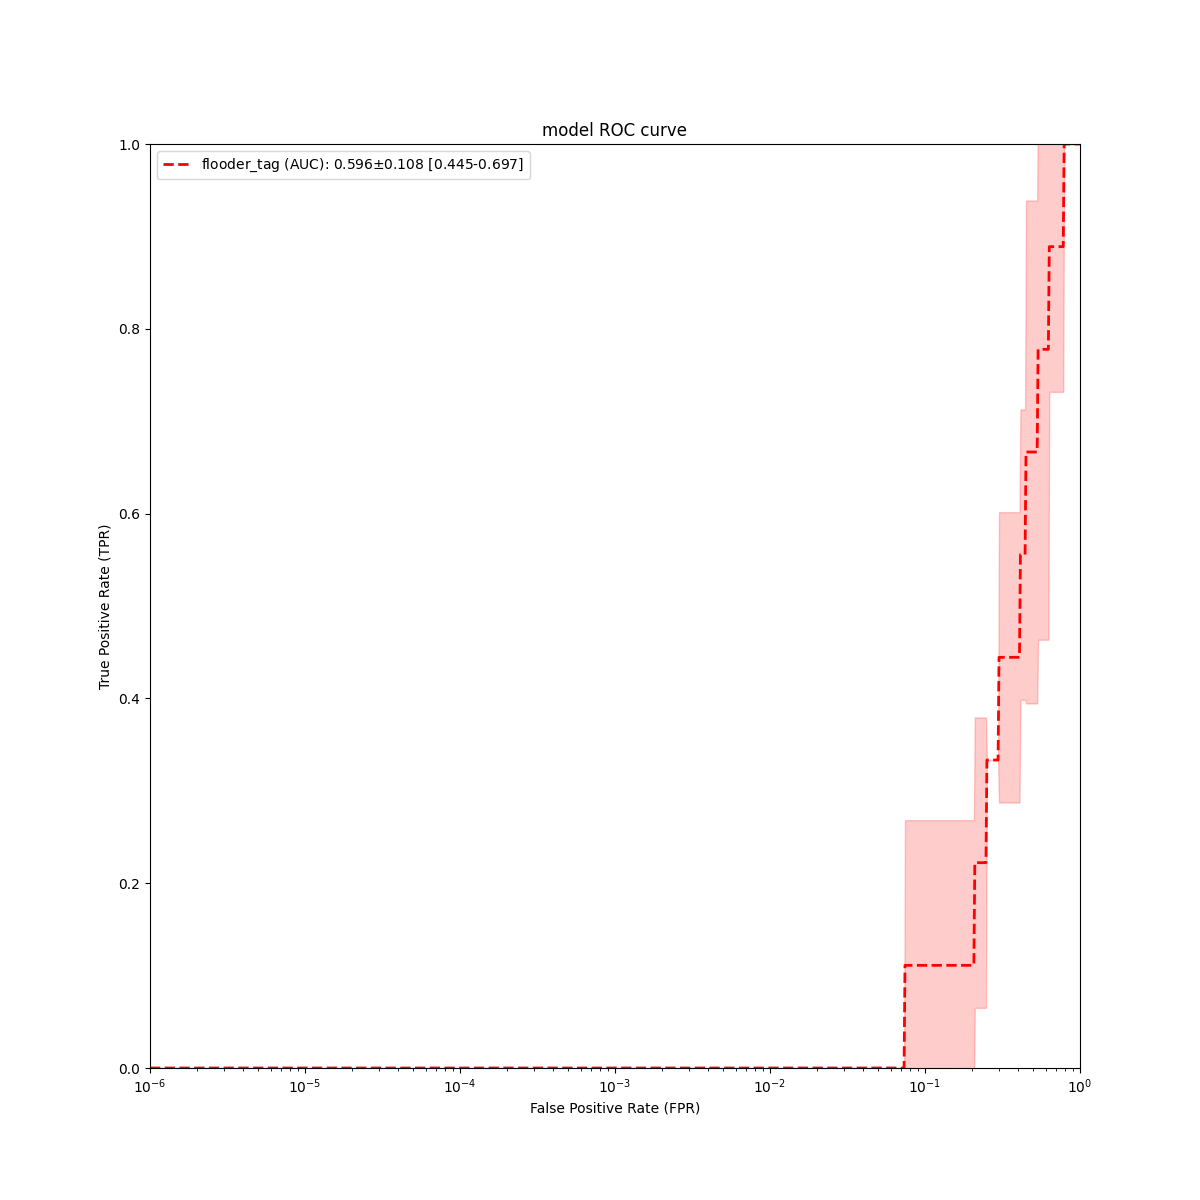
\includegraphics[width=0.6\textwidth]{./results/flooder_tag_roc_aloha.png}
        \vspace*{-0.2cm}
        \caption[Flooder Tag prediction task ALOHA ROC curve]{ROC curve and AUC statistics of \textBF{ALOHA} model for the \textbf{Flooder Tag}. The line represents the \textit{mean} TPR at a given FPR, while the shaded region represents the \textit{standard deviation}. Statistics were computed over \textBF{2} training runs, each with random parameter initialization.}
        \label{fig:flooderTagRocAloha}
    \end{figure}
}

\newcommand{\flooderTagRocProposedMethod}{
    \begin{figure}[H]
        \vspace*{-0.5cm}
        \centering
        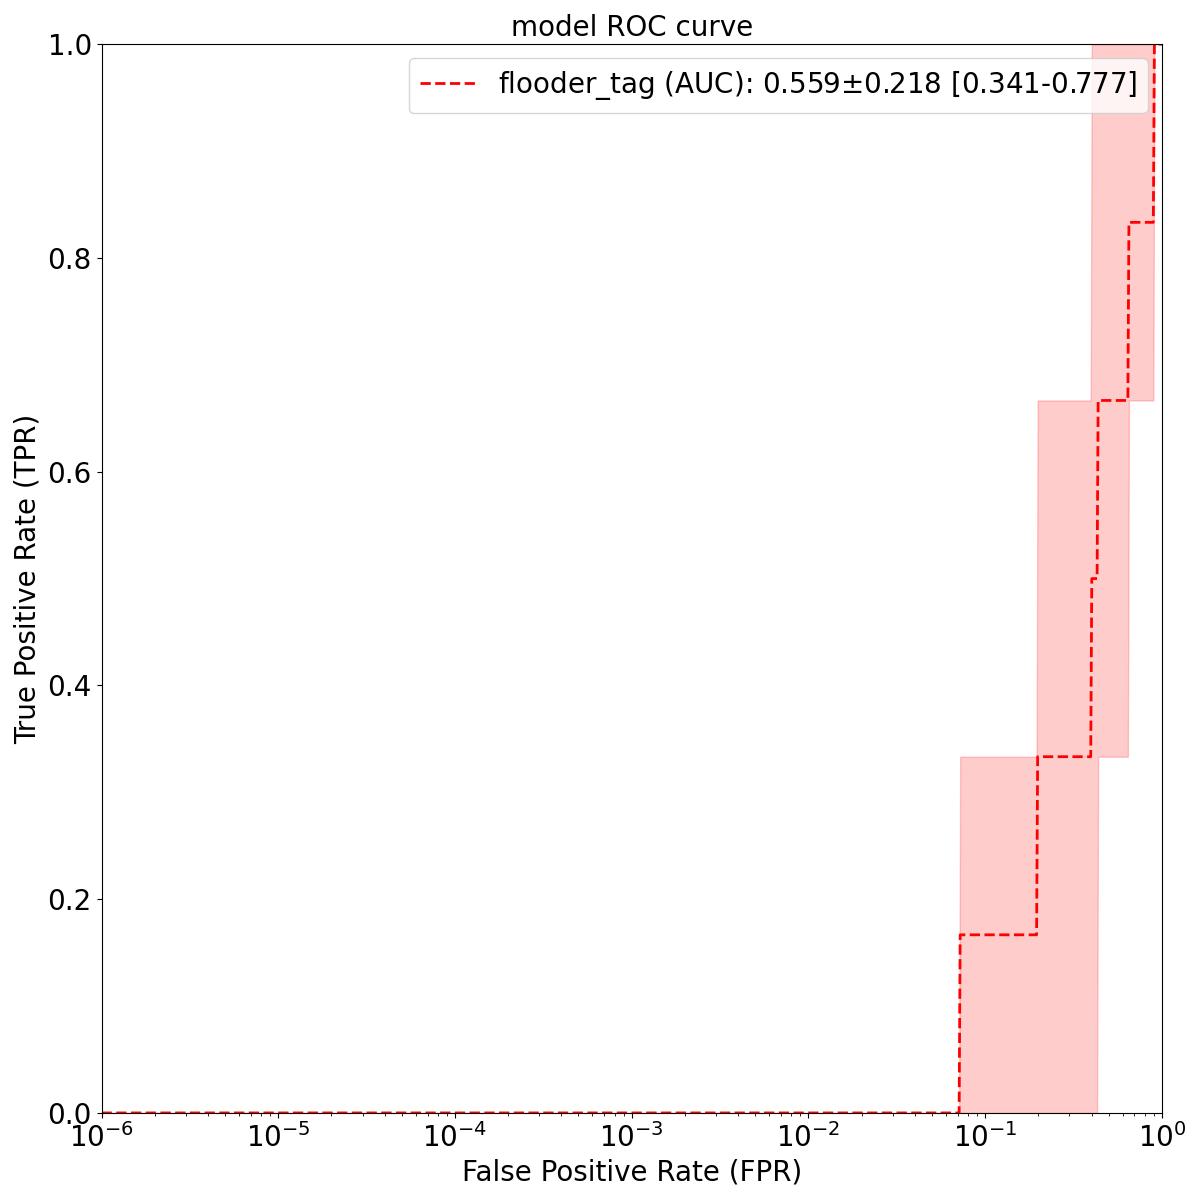
\includegraphics[width=0.6\textwidth]{./results/flooder_tag_roc_proposedModel.png}
        \vspace*{-0.2cm}
        \caption[Flooder Tag prediction task Proposed Model ROC curve]{ROC curve and AUC statistics of \textBF{Proposed Model} for the \textbf{Flooder Tag}. The line represents the \textit{mean} TPR at a given FPR, while the shaded region represents the \textit{standard deviation}. Statistics were computed over \textBF{2} training runs, each with random parameter initialization.}
        \label{fig:flooderTagRocProposedModel}
    \end{figure}
}
